\documentclass[11pt]{article}
\usepackage[margin=1in]{geometry}
\usepackage{amsmath,amssymb}
\usepackage{graphicx}
\graphicspath{{figures/}}
\usepackage{booktabs}
\usepackage[colorlinks=true,linkcolor=blue,citecolor=blue,urlcolor=blue]{hyperref}

\title{Benchmark notes for \texttt{lebedev\_em}}
\author{Shari Moskow \thanks{Department of Mathematics, Drexel University.
Prepared with assistance from Claude (Anthropic).}}
\date{July 20, 2026 (revised)}

\newcommand{\sdot}{\dot\sigma}

\begin{document}
\maketitle

\begin{abstract}
These notes document the benchmarks for the \texttt{lebedev\_em} solver, a
Python implementation of the Lebedev staggered-grid finite-difference scheme
of Davydycheva, Druskin \& Habashy \cite{DDH03} (DDH03) for the
frequency-domain Maxwell equations in 3-D anisotropic inhomogeneous media.
Two inhomogeneous benchmarks are presented. The first, a two-half-space model
with a $10\times$ conductivity contrast, is validated against the exact
Sommerfeld-integral solution: the four-cluster Lebedev average attains
$\approx 1\%$ accuracy in the conductive half-space, and cluster averaging
reduces the single-cluster error fivefold. The second reproduces the
configuration of DDH03 Figure~9 --- a resistive borehole with an invaded
zone crossing a thin $75^\circ$ dipping anisotropic layer with
$\sigma_N = \sigma_T/200$ --- and matches the published curves at the
few-percent level with unit dipole moment and no fitted parameters,
\emph{identically at every grid resolution}, using either the DDH03 eq.-(8/9)
laminate (Backus) averaging or the nodal homogenization of \cite{MDHLD99} in
a fully coupled four-cluster solve. A three-level refinement study shows that
the two averaged schemes agree with each other to $\approx 1\%$ and are
resolution-independent (reproducing DDH03's own $k=6$ vs.\ $k=12$
insensitivity), whereas na\"ive pointwise sampling of the conductivity is off
by $20\%$ or more at every practical resolution and converges only slowly.
The study also identifies a subtlety of the published model that an earlier
version of these notes got wrong: the invasion annulus ($R = 0.6$ m), although
it carries the background conductivity, \emph{replaces the anisotropic layer}
near the borehole, so the layer is present only at $r \ge 0.6$ m.
\end{abstract}

\section{The solver and its verification chain}

\texttt{lebedev\_em} discretizes the frequency-domain Maxwell system (time
convention $e^{-i\omega t}$)
\begin{equation}
\nabla\times \mathbf{E} = i\omega\mu\mathbf{H}, \qquad
\nabla\times \mathbf{H} = \sdot\,\mathbf{E} + \mathbf{J},
\qquad \sdot = \sigma - i\omega\varepsilon,
\end{equation}
on Lebedev's staggered grid, which supports full $3\times3$ conductivity
tensors without interpolation and splits into four Yee-like clusters. The
implementation follows the complete DDH03 methodology: distributed sources in
all four clusters satisfying their eq.~(7) (unit total weight, centroid at
the physical source), mixed electric/magnetic boundary conditions assigned
per cluster so that domain-truncation errors cancel in the four-cluster
average, interpolate-then-average field extraction, optimal geometric
transverse grids ($\alpha = e^{\gamma\pi/\sqrt{k}}$, $\gamma = 1/\sqrt2$)
with a hybrid axial grid (fine equidistant near source and receivers,
geometric beyond), and sub-cell homogenization of interface-cut cells.

The verification chain proceeds from analytic anchors outward: the discrete
operators are unit-tested (symmetry of the curl--curl system in its
volume-weighted inner product, source weight and centroid conditions on
nonuniform grids); the solver reproduces the closed-form magnetic-dipole
solution in homogeneous isotropic media at both 2.5~kHz and 52.65~kHz to a
few percent at moderate resolution; and the two inhomogeneous benchmarks
below add a sharp material interface and a thin anisotropic structure. All
results are per unit dipole moment ($1$~A$\cdot$m$^2$) in SI units, with no
calibration constants anywhere in the chain.

\section{Benchmark 1: two half-spaces, $10\times$ contrast}

\paragraph{Model.} A unit vertical electric dipole (VED) at the origin in
\[
\sigma(z) = \begin{cases} 0.1 \text{ S/m}, & z < 4\text{ m},\\
1.0 \text{ S/m}, & z \ge 4 \text{ m},\end{cases}
\qquad f = 2500 \text{ Hz},
\]
with receivers on the $z$-axis, $z\in[0.5,\,7.5]$ m, straddling the contact.
The reference is the exact Sommerfeld-integral solution for $E_z$
(implemented in \texttt{analytics.py} and independently verified: it reduces
to the closed-form homogeneous solution when $\sigma_1=\sigma_2$ to
$3\times10^{-14}$ relative, and satisfies the normal-current continuity
$\sigma_1 E_z^- = \sigma_2 E_z^+$ at the contact).

\paragraph{Grid.} Optimal geometric transverse grids with $k=3$
($M_x=M_y=12$), hybrid axial grid with $\Delta z = 0.0625$ m near the source
($M_z=160$, $\approx 41$k complex degrees of freedom).

\paragraph{Results.} Figure~\ref{fig:twolayer} shows $|E_z|$ on the axis, the
pointwise deviation from the analytic solution, and the contact effect.

\begin{itemize}
\item In the conductive half-space ($z \ge 4$ m), across the $10\times$ jump,
the RMS relative error of $\mathrm{Re}\,E_z$ is $\mathbf{1.0\%}$.
\item The overall RMS error ($5.6\%$) is dominated by the near-source region,
where the transverse domain is only $0.3\,\delta_1$ wide; the \emph{same}
error appears in a homogeneous control run (RMS $5.7\%$), so the interface
itself contributes essentially nothing --- the scheme crosses the contact
cleanly.
\item The physical structure at the contact is captured quantitatively: the
two-layer/homogeneous ratio rises to $1.65$ just above the contact and drops
to $\approx 0.18$ below it, matching the analytic curve point by point.
\item Cluster averaging matters: a single cluster (C000) gives RMS $29.9\%$;
the four-cluster Lebedev average reduces this to $5.7\%$ --- DDH03's
error-cancellation mechanism at work in an inhomogeneous medium.
\end{itemize}

\begin{figure}[htbp]
\centering
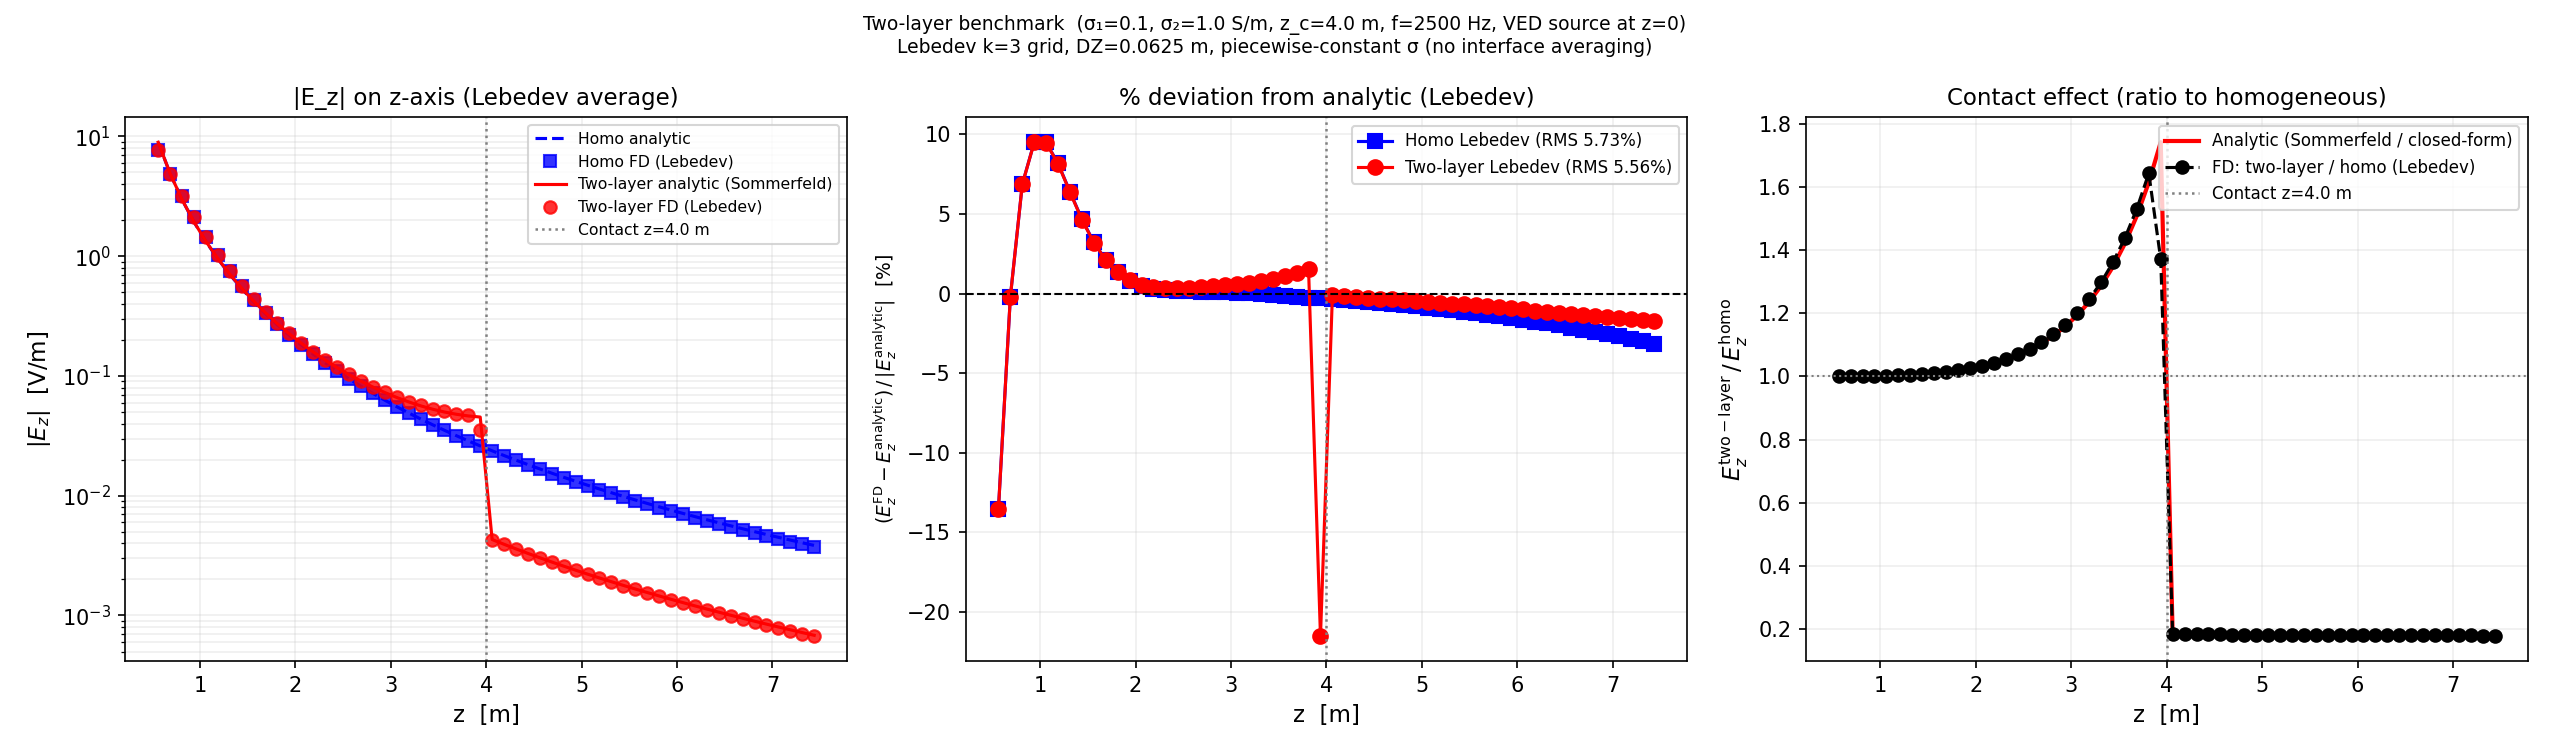
\includegraphics[width=\textwidth]{benchmark_two_layer.png}
\caption{Two-half-space benchmark ($\sigma_1=0.1$, $\sigma_2=1.0$ S/m,
contact at $z_c=4$ m, $f=2500$ Hz). Left: $|E_z|$ on the axis, FD (symbols)
vs.\ analytic (lines). Center: pointwise percent deviation. Right: contact
effect --- two-layer to homogeneous ratio, FD (black) vs.\ Sommerfeld
analytic (red). The isolated spike in the center panel sits at the contact
node itself, where $E_z$ is discontinuous and a pointwise comparison is
ill-posed.}
\label{fig:twolayer}
\end{figure}

\section{Benchmark 2: thin dipping anisotropic layer crossed by a borehole}

\paragraph{Model.} The configuration of DDH03 Figure~9
(Fig.~\ref{fig:medium}): a homogeneous background $\sigma = 0.1$ S/m; a
resistive borehole column ($\sigma = 0.05$ S/m, $R = 0.1$ m) along the
$z$-axis; an invaded zone ($\sigma = 0.1$ S/m, $R = 0.6$ m); and a thin
dipping anisotropic layer of $0.25$ m normal thickness, dip $75^\circ$, with
transverse conductivity $\sigma_T = 0.1$ S/m and normal conductivity
$\sigma_N = \sigma_T/200$ --- a $1{:}200$ contrast confined to a layer
thinner than most local grid cells. The layer crosses the borehole axis over
$z \in [-1.93, -0.95]$ m. The source is a $z$-directed unit magnetic dipole
at the origin, $f = 52.65$ kHz; the observable is $\mathrm{Im}\,B_z$ on the
axis. Two cases are run: \emph{no layer} (borehole only) and
\emph{resistive layer}.

A modelling subtlety, corrected in this revision, turned out to control the
comparison. The invasion annulus carries the \emph{same} conductivity as the
background, and an earlier version of these notes therefore omitted it. But
in the DDH03 model family (cf.\ their Figs.~6--7, where the invasion visibly
punches through the layered formation) the invaded zone \emph{replaces} the
formation near the wellbore: the anisotropic layer exists only for
$r \ge 0.6$ m. Because the induction tool is most sensitive precisely in
that near-axis region, the two readings differ enormously --- modelling the
layer all the way in to the borehole wall increases the layer's attenuation
of $\mathrm{Im}\,B_z$ from $\approx 27\%$ to $\approx 51\%$ (geometric mean
over the receivers) and cannot be reconciled with the published curve by any
choice of scheme or resolution.

\begin{figure}[htbp]
\centering
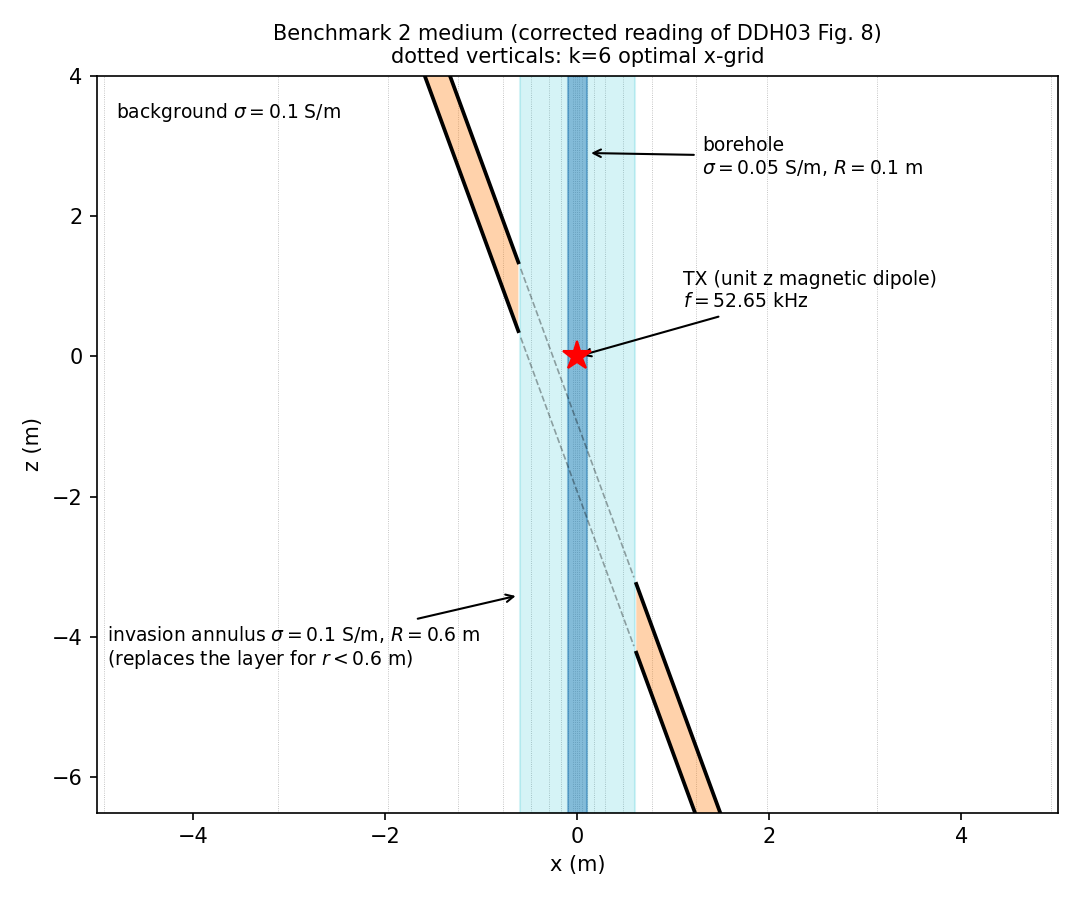
\includegraphics[width=0.72\textwidth]{fig9_medium.png}
\caption{Benchmark 2 medium, $x$--$z$ section (corrected reading of DDH03
Fig.~8). The invasion annulus ($\sigma = 0.1$ S/m, $R = 0.6$ m) coincides
with the background conductivity but replaces the anisotropic layer for
$r < 0.6$ m, so the layer (orange) is an annular structure. Dotted verticals
show the $k=6$ optimal transverse grid.}
\label{fig:medium}
\end{figure}

\paragraph{Method.} Full DDH03 methodology as in \S1: optimal transverse
grids, hybrid axial grid with the source exactly on a grid node,
four-cluster sources and mixed boundary conditions, exact-geometry sub-cell
homogenization (exact interface normals and volume fractions from the
analytic geometry) by either the DDH03 eq.-(8/9) laminate (``Backus'')
scheme or the nodal scheme of \cite{MDHLD99}, a \emph{single fully coupled}
sparse iterative solve (the off-diagonal conductivity couples the four
clusters; solving them separately under-counts the anisotropy-generated
cross-components), and interpolated four-cluster averaging at the exact
receiver positions. Three refinement levels are run, scaling the transverse
minimal step and the axial spacing together while growing $k$ to hold the
domain reach: L1 ($h_{\min}=0.05$ m, $k=6$, $\approx 121$k unknowns --- the
published-comparison grid), L2 ($h_{\min}=1/30$ m, $k=7$, $\approx 223$k),
and L3 ($h_{\min}=0.025$ m, $k=8$, $\approx 368$k). All iterative solves
converged to $10^{-8}$ relative residual.

\paragraph{Absolute calibration of the reference.} The published ``no
layer'' curve serves double duty: comparing it to the closed-form
homogeneous-medium solution shows agreement within $1$--$8\%$ (the deficit
appearing near the source, consistent with the borehole's local reduction of
the field). This confirms that the published figure is in absolute SI units
per unit dipole moment, so the comparison below involves no free scale.

\paragraph{Results.} Figure~\ref{fig:fig9curves} overlays the computed
curves at the finest grid (lines) on the values digitized from the published
figure (symbols).

\begin{itemize}
\item \textbf{No layer:} agreement within $0.3$--$4.5\%$ at every receiver
(geometric-mean ratio $1.021$ Backus, $1.019$ nodal at L3; log-scatter
$1.1\%$), improving steadily with refinement ($1.035$ at L1). This confirms
the absolute normalization and sets the accuracy floor of the digitization
itself at the $1$--$2\%$ level.
\item \textbf{Resistive layer (invaded model):} agreement within
$3$--$12\%$ (geometric-mean ratio $1.070$ Backus, $1.077$ nodal at L3;
log-scatter $2\%$), and --- crucially --- \emph{flat across all three
refinement levels}: the Backus ratio moves only $1.085 \to 1.073 \to 1.070$
from L1 to L3, and Backus and nodal agree with each other to better than
$1.2\%$ at every receiver. In the grid-calibration-free attenuation measure
(geometric mean of the layer/no-layer ratio over the receivers) the published
figure gives $0.697$ and the averaged schemes give $0.729$--$0.742$ at every
level. The residual few percent is consistent with digitization error: both
the layer's axis intercepts ($-0.95$/$-1.93$ m) and the published values
themselves are read off the printed figure.
\end{itemize}

\begin{figure}[htbp]
\centering
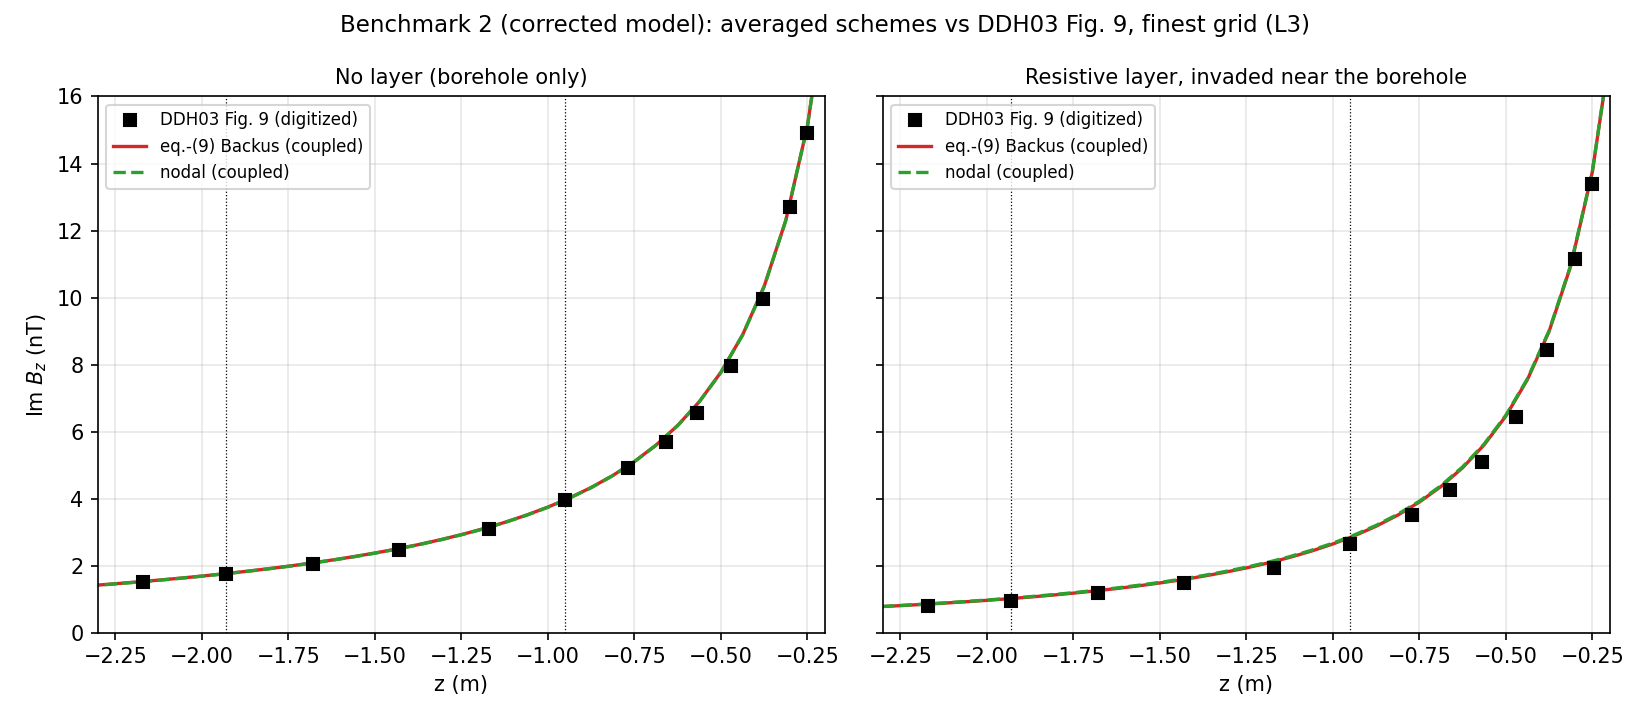
\includegraphics[width=\textwidth]{fig9_ours_vs_digitized.png}
\caption{Benchmark 2: $\mathrm{Im}\,B_z$ on the axis at the finest grid
(L3). Lines: \texttt{lebedev\_em}, coupled solve with eq.-(9) Backus (solid
red) and nodal (dashed green) averaging --- the two are indistinguishable at
this scale. Symbols: values digitized from DDH03 Fig.~9. Unit dipole moment
on both sides; no fitted constants. Dotted verticals mark where the layer
crosses the axis.}
\label{fig:fig9curves}
\end{figure}

\paragraph{Refinement study: averaging is required, and the model matters
more than the scheme.} Figure~\ref{fig:refinement} summarizes the
three-level refinement study for both readings of the model and all three
sub-cell treatments. Three conclusions:

\begin{enumerate}
\item \textbf{The two averaged schemes are resolution-independent and
equivalent.} On the correct (invaded) model, Backus and nodal sit within
$\approx 7\%$ of the published curve at every level and within $\approx 1\%$
of each other --- reproducing DDH03's own observation that their $k=6$ and
$k=12$ curves ``can hardly be distinguished,'' a property that only holds
for averaging schemes. This is the frequency-domain counterpart of the
thin-resistive-structure results of \cite{MDHLD99}: the sub-cell layer is
captured by homogenization, not by resolution.
\item \textbf{Pointwise sampling is inadequate at any practical resolution.}
On the invaded model it overshoots the published curve by $26\%$ at L1 and
is still $22\%$ high at L2; in a controlled tilted-slab study with the same
layer material it remains $23\%$ high even at $t/h = 2.6$ and converges only
slowly from above.
\item \textbf{The earlier contrary conclusion was a model artifact.} On the
\emph{uninvaded} model (layer extending to the borehole wall), pointwise at
the published-comparison grid happens to land on the digitized curve
(attenuation $0.698$ vs.\ the paper's $0.697$) --- a double coincidence in
which pointwise's failure to see the sub-cell layer imitates the genuinely
absent near-axis layer of the true model. Refinement unmasks it: the
pointwise curve drifts steadily down through and past the published values
($1.036 \to 1.008 \to 0.982$ of the paper from L1 to L3, still falling),
while the averaged schemes on the same wrong model sit $30\%$ low at every
level. No scheme reproduces the published curve on the uninvaded model;
both averaged schemes reproduce it on the invaded one.
\end{enumerate}

\begin{figure}[htbp]
\centering
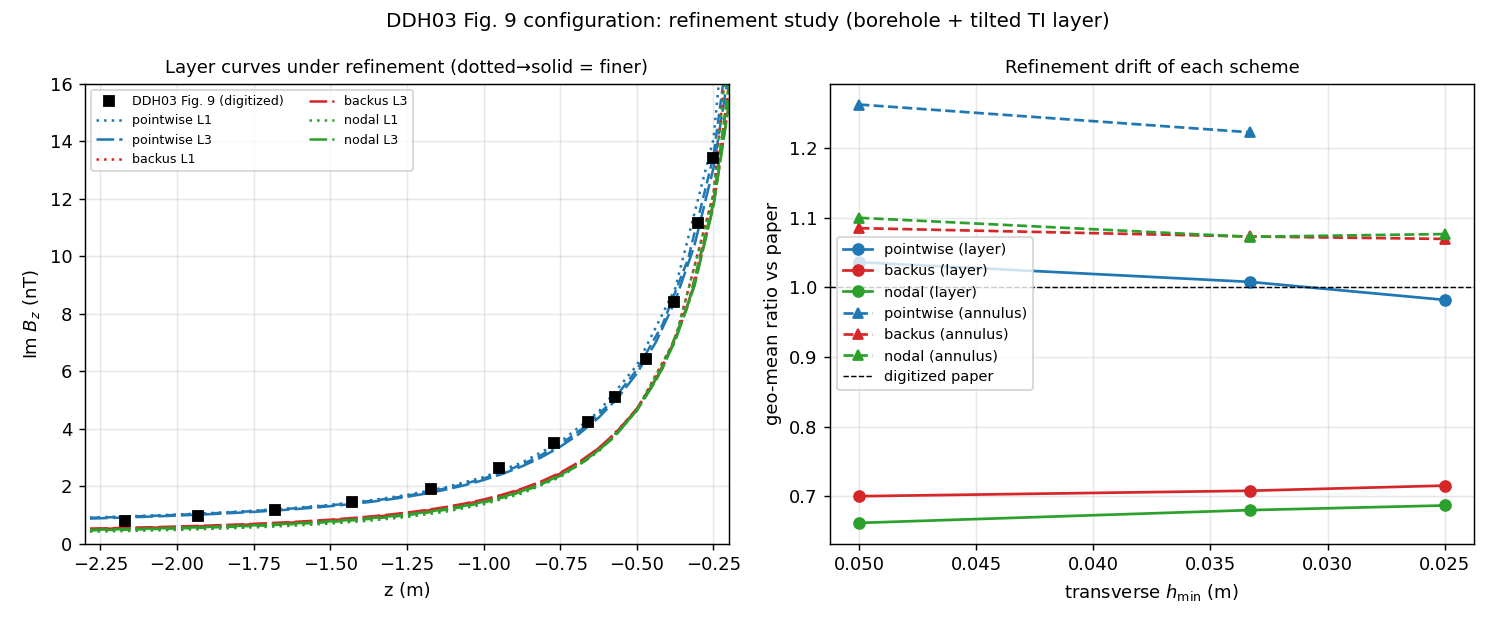
\includegraphics[width=\textwidth]{fig9_model_refinement.png}
\caption{Three-level refinement study of Benchmark 2. Left: the
resistive-layer curves for the uninvaded model under refinement. Right:
geometric-mean ratio to the digitized published values for each scheme, on
the uninvaded (``layer,'' circles) and invaded (``annulus,'' triangles)
models. The averaged schemes on the invaded model (red/green triangles) are
flat at $\approx 1.07$; pointwise is resolution-dependent on either model.}
\label{fig:refinement}
\end{figure}

\section{Remarks}

The two benchmarks are complementary: Benchmark~1 has an exact external
reference and tests the sharp-interface machinery and cluster averaging;
Benchmark~2 tests the full anisotropic pipeline --- tilted tensors, a
borehole crossing a thin high-contrast layer, homogenization, the coupled
four-cluster solve --- against independently published curves whose absolute
normalization we verified analytically, and its refinement study
additionally validates the resolution-independence that is the central claim
of the DDH03 averaging approach. Both succeed with unit dipole moment and no
adjustable constants.

Benchmark~2's history is itself instructive. The earlier version of these
notes reported that only the nodal scheme (run in a then-current sequential
per-cluster mode) reproduced the published curve. Subsequent work replaced
the sequential solves by the fully coupled solve, verified the eq.-(9)
averaging, the coupled off-diagonal operator, and both averaged schemes
against analytic and refinement ground truths in a chain of controlled
tests (tilted whole-space, single tilted interface, tilted sub-cell slab),
and traced every remaining discrepancy with the published figure to the
model-transcription error described in \S3: the omitted invaded zone. The
lesson we would pass on: when a benchmark against a digitized figure
disagrees, refine the grid before trusting the match --- the scheme that
agreed at the published resolution was the one that was wrong.

Work in progress: the deviated-borehole model of DDH03 Figs.~6--7 (borehole,
invasion zone, and a $60^\circ$ dipping anisotropic half-space) reproduces
the published curve \emph{shapes} precisely but not yet their amplitudes.
The discrepancy had independently been localized to the treatment of the
invasion zone in that figure; in light of the Benchmark-2 resolution ---
the invaded zone replaces the formation, including any anisotropic layers it
crosses --- that model is being revisited and is omitted from these notes
until it is settled.

\begin{thebibliography}{9}
\bibitem{DDH03} S.~Davydycheva, V.~Druskin, T.~Habashy,
\emph{An efficient finite-difference scheme for electromagnetic logging in 3D
anisotropic inhomogeneous media}, Geophysics \textbf{68}(5):1525--1536, 2003.
\bibitem{MDHLD99} S.~Moskow, V.~Druskin, T.~Habashy, P.~Lee,
S.~Davydycheva, \emph{A finite difference scheme for elliptic equations with
rough coefficients using a Cartesian grid nonconforming to interfaces},
SIAM J.\ Numer.\ Anal.\ \textbf{36}:442--464, 1999.
\end{thebibliography}

\end{document}
